Asymmetric encryption provides confidentiality, while digital signatures provide integrity. In essence, a \textbf{digital signature} (or simply signature) is a sequence of bytes created through a dedicated asymmetric algorithm taking as input some data and a private key (\Cref{figure:digital_signature_creation_and_verification}). The act of creating a signature over some data is also referred to as \textit{signing the data}. The public key associated with the aforementioned private key can be used for \textit{verifying the signature}, thus verifying the integrity of the data.


\subsection{Digital Signatures and Security Properties}\label{sec:digital_signatures:security_properties}

By themselves, digital signatures provide integrity only. However, depending on how (public keys corresponding to) private keys used to create signatures are bonded to parties, signatures may provide further security properties such as sender authenticity and non-repudiation (\Cref{sec:security_properties}). The two main mechanisms for binding public keys to parties are \glspl{pki} and the \gls{wot} (\Cref{sec:binding_keys_to_parties,sec:binding_keys_to_parties:wot}, respectively).

In detail, a digital signature provides:
\begin{itemize}
	\item \textit{public verifiability} if anyone within a system can access the signature, the associated data, and the public key required to verify the signature;
	\item \textit{sender authenticity} if the key pair used to create the signature --- that is, the public key of the key pair --- is somehow reliably bonded to a party. Usually, the party actively claims possession of the key pair and this claim is typically endorsed by one or more parties (which may be trusted by everyone within the system);
	\item \textit{unforgeability} if attackers cannot produce signatures that authenticate to --- that is, seem to have been created by --- other parties without having the parties' private key;
	\item \textit{non-repudiation} if it already provides sender authenticity, unforgeability, and the key pair used to create the signature --- more precisely, the private key of the key pair --- has always been under the sole control of the owner party.
\end{itemize}

\remarkBlock{Digital signatures and deniability}{Typically, digital signatures are not used when deniability is required; in such cases, \glspl{mac} (\Cref{sec:symmetric_cryptography:mac}) are used instead.}

\begin{figure}[t!]
	\begin{center}
		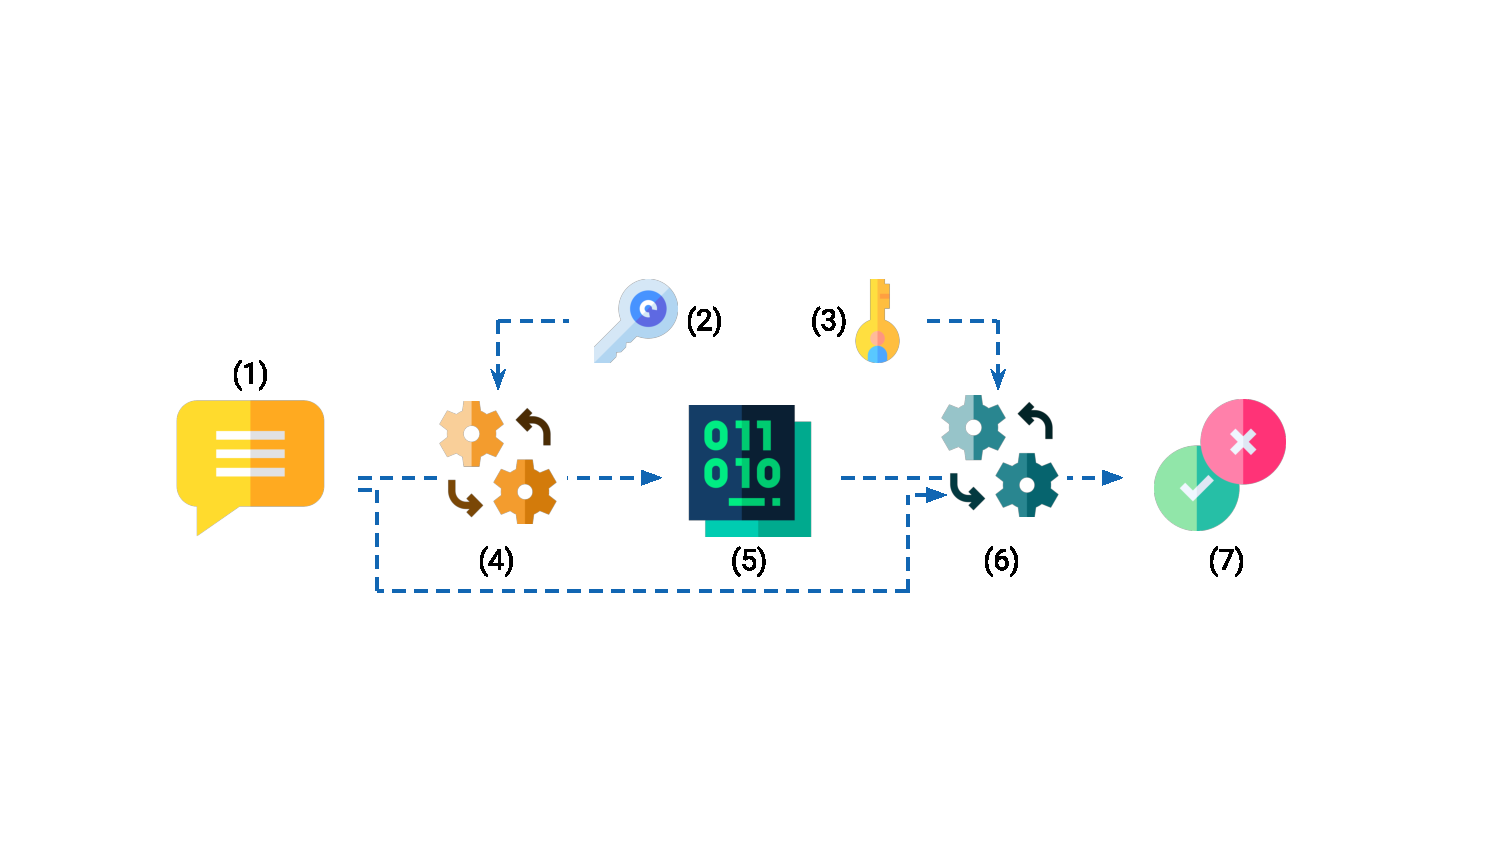
\includegraphics[trim={3cm 4cm 3.5cm 4.5cm},clip,width=0.75\linewidth]{resources/pdf/digital_signature_creation_and_verification.pdf}
		\caption{The process of creating and verifying digital signatures. The data to be signed (1) --- any sequence of bytes of arbitrary length --- and a private key (2) are given as input to the signature creation algorithm (4) which returns as output the signature (5). The signature verification algorithm (6) takes as input the data (1), the signature (5), and the public key (3) associated with the private key (1), and returns as outcome a boolean value (7) --- either the signature is valid or it is not.}
		\label{figure:digital_signature_creation_and_verification}
	\end{center}
\end{figure}